\documentclass[10pt,twocolumn,letterpaper]{article}

\usepackage{cvpr}
\usepackage{times}
\usepackage{epsfig}
\usepackage{graphicx}
\usepackage{amsmath}
\usepackage{amssymb}

% Include other packages here, before hyperref.

% If you comment hyperref and then uncomment it, you should delete
% egpaper.aux before re-running latex.  (Or just hit 'q' on the first latex
% run, let it finish, and you should be clear).
%\usepackage[pagebackref=true,breaklinks=true,letterpaper=true,colorlinks,bookmarks=false]{hyperref}

\cvprfinalcopy % *** Uncomment this line for the final submission

\def\cvprPaperID{1} % *** Enter the CVPR Paper ID here
\def\httilde{\mbox{\tt\raisebox{-.5ex}{\symbol{126}}}}

% Pages are numbered in submission mode, and unnumbered in camera-ready
\ifcvprfinal\pagestyle{empty}\fi
\begin{document}

%%%%%%%%% TITLE
\title{ Investigation of Sign Detection Algorithms}

\author{Brian Fehrman\\
SDSM\&T\\
501 E. Saint Joseph Street\\
{\tt\small bcfehrman@gmai1.com}
% For a paper whose authors are all at the same institution,
% omit the following lines up until the closing ``}''.
% Additional authors and addresses can be added with ``\and'',
% just like the second author.
% To save space, use either the email address or home page, not both
\and
Ross Hoyer\\
SDSM\&T\\
501 E. Saint Joseph Street\\
{\tt\small ross.hoyer@gmail.com}
}

\maketitle
\thispagestyle{empty}

%%%%%%%%% ABSTRACT
\begin{abstract}
In this work we will explore algorithms used for sign recognition and attempt to improve upon them. The main goals are to detect stop signs and one-way street signs as we feel that missing either of these could prove to be disastrous for a driver. Recognition of other signs such as speed limit signs and do-not-enter signs will also be investigated if time permits. The testing for the different methods will be done using video feed that is recorded from a GoPro camera. This camera has been mounted in a daily driven car to capture realistic driving footage for the area. After bench marking the algorithms on a PC it will be determined if they can be feasibly ported to a mobile platform such as the Android. If portability is possible then the methods will be combined in to a single program that can run on a phone with a camera and potentially aid drivers.

\end{abstract}

%%%%%%%%% BODY TEXT


\section{Introduction}
Sign detection has been a popular topic for awhile now \cite{Piccioli1994, Mace1984}. For our Fall 2012 Computer Vision Graduate Student project we will be exploring this topic further. The signs we are specifically interested in are stop signs and one-way street signs which are some of the most important signs to notice in terms of safety. We will look at some of the more recent methods that have been used to quickly recognize signs from a video feed. Ways to improve upon these algorithms will be researched. If fast enough, these improved algorithms could be capable of assisting drivers by the use of a mobile phone camera. Ultimately, highly reliable sign recognition algorithms will most likely be needed if automated cars are to become a reality.

%----------------------------1---------------------------------------------
\section{Recent Work}

In Shojania's work he explored detection of yield signs, stop signs, and red-bordered circular signs. He first segmented the image based upon color and then detected features by using convolution masks. He then applied geometric constraints to determine if a sign had been found \cite{Shojania2007}. 

Song et. al. investigated multiple algortihms for the detection of stop signs. They found that using HAAR features with decisions trees did not produce good results. They next tried a Histogram of Oriented Gradients approach which proved to work better than the HAAR approach. Lastly, they tried template matching using various templates sizes with varying blur effects and found that to work the best out of the three methods that they implemented \cite{Song2008}.

Lafuente-Arroyo et. al. approached the sign detection problem by first segmenting the image based upon Hue, Saturation, and Intensity versus the typical RGB filtering that is used and found this to be more robust to changes in lighting. To make it work well with white signs as well, however, they had to additionally use a method to find achromatic colors. Pixels were then grouped based on color. They then extracted features based upon a Distance to Bounding box which just measured the distance from the detected object's edges to the box. A support vector machine was then used to determine if the object was possibly a sign \cite{Lafuente-Arroyo2010}. 


\section{Proposed Approach}
Our work will involve the use of OpenCV to solve the sign detection problem. The testing will be performed on recorded video footage from a GoPro camera that has been mounted in one of the author's cars. The author has driven multiple paths around town to get a variety of footage and under different environmental conditions (cloudy, sunny, etc.). We will first run a corner detection algorithm on a given frame to find good features within the image. We will then look for groups of features that potentially form the shape of a desired sign. From there, we can extract a feature region and attempt to match it with signs that are of the same shape. Our main goal is to detect stop signs (Figure \ref{fig:stop_sign}) and one-way signs which actually come in two varieties (Figures \ref{fig:one-way1} and \ref{fig:one-way2}). We are only considering the United States versions of these signs and do realize that other varieties exist in other countries. The detection methods will be run on a PC and we will determine the execution time to see if porting to a mobile device will be feasible. If time allows then we will look at some other signs such as do-not-enter and speed limit signs.


\begin{figure}[ht!]
\centering
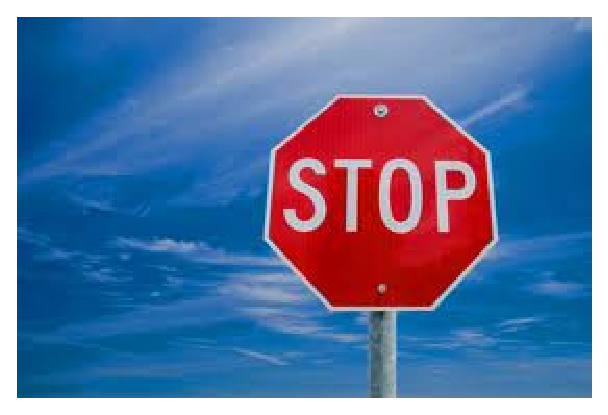
\includegraphics[width=0.3\textwidth]{img/stop}
\caption{Stop sign}
\label{fig:stop_sign}
\end{figure}

\begin{figure}[ht!]
\centering
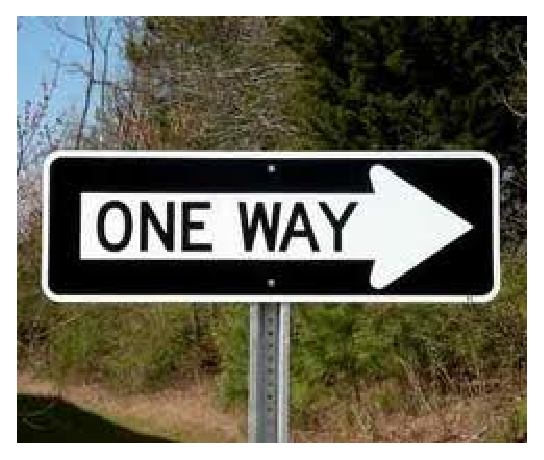
\includegraphics[width=0.3\textwidth]{img/one-way1}
\caption{One type of one-way sign}
\label{fig:one-way1}
\end{figure}

\begin{figure}[ht!]
\centering
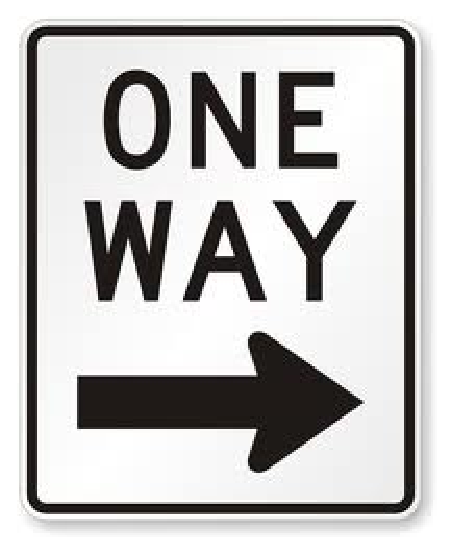
\includegraphics[width=0.2\textwidth]{img/one-way2}
\caption{Another type of one-way sign}
\label{fig:one-way2}
\end{figure}


{\small
\bibliographystyle{ieee}
\bibliography{egbib}
}

\end{document}
